\documentclass[12pt,a4paper,fontset=mac]{ctexart}
\usepackage[margin=2.2cm]{geometry}
\usepackage{graphicx,booktabs,amsmath,float,xcolor,listings}
\usepackage{longtable,array,caption}
\usepackage[hidelinks]{hyperref}
\graphicspath{{images/}}
\setlength{\emergencystretch}{2em}
\setlength{\parskip}{0.25em}
\renewcommand{\arraystretch}{1.18}
\captionsetup{font=small,labelfont=bf}
\lstset{language=Python,basicstyle=\ttfamily\footnotesize,
 keywordstyle=\color{blue!70!black},commentstyle=\color{green!40!black},
 stringstyle=\color{orange!60!black},showstringspaces=false,breaklines=true,
 breakatwhitespace=false,columns=fullflexible,keepspaces=true,frame=single,
 tabsize=4,numbers=left,numberstyle=\tiny\color{gray},numbersep=6pt,
 xleftmargin=1em,aboveskip=0.8em,belowskip=0.8em}
\newcommand{\reporttitle}{实验一：性能评价与仿真方法学}
\newcommand{\subtask}{ROI、CPU 模型、排序保真度与工作负载规模}
\newcommand{\authname}{姓名}
\newcommand{\authid}{学号}
\newcommand{\class}{班级}
\title{\reporttitle\\[0.4em]\large\subtask}
\author{\small\authname：\underline{李祥熙}\quad
\authid：\underline{2234412799}\quad\class：\underline{计算机2301}}
\date{2026年10月30日}
\begin{document}
\maketitle
\begin{abstract}
本实验使用 gem5 的 RISC-V SE 模式，围绕 int8 神经网络推理程序 qnn，研究测量区间、代码布局、CPU 模型及工作负载规模对性能评价的影响。实验完成任务 1--5，并以随机指针追逐完成选做任务 6。主要结果为：初始化段仅占全程序指令数的 16.25\%，却占 40.26\% 的周期；移除未对齐程序的 ROI 标记后，指令数仅增加 19 条，全程序周期却变为约 3.05 倍；在 qnn 上，Timing、Minor 与 O3 对大容量 L1D 分别给出变慢、近似不变与变快三种结论。改用依赖访存链后，三个模型均选择 128 KiB。最终选择 O3 及 8 个 qnn 样本作为后续实验默认配置，以周期数衡量性能，以主机耗时衡量仿真成本，并将排序保真度作为模型适用性的关键判断标准。
\end{abstract}
\clearpage
\tableofcontents
\newpage

\section{实验目的}
\begin{itemize}
\item 理解目标程序的模拟执行时间与主机运行模拟器所需时间的区别，正确使用指令数、周期数、IPC 和仿真速率。
\item 通过同一程序的分段统计量化初始化与收尾成本，掌握 ROI 的划分方法，分析跨二进制相减和代码布局带来的测量干扰。
\item 比较 Atomic、Timing、Minor、O3 四个 CPU 模型，判断简化模型能否保留设计方案的性能排序。
\item 在稳定执行行为和仿真成本之间选择合适的工作负载规模，并通过另一负载检验结论的适用范围。
\end{itemize}

\section{实验过程}
\subsection{实验环境与数据来源}
主机为 Apple M4、10 核、16 GiB 内存，操作系统为 macOS 27.0.1。gem5 版本为 25.0.0.1，目标 ISA 为 RISC-V，Python 版本为 3.11.15。程序以 Linux/glibc 静态可执行文件形式交叉编译；macOS 上通过已有 Docker/Colima 工具链完成编译，gem5 在主机上原生运行。仿真采用 SE 模式，不启动完整操作系统，由模拟器代办目标程序的系统调用。

表~\ref{tab:config} 给出默认模拟配置。这里的 2 GHz 是目标处理器频率，与主机时钟频率无关；命令中的 \texttt{kB} 按 gem5 实际解释为二进制容量，下文统一写作 KiB。
\begin{table}[H]\centering\small
\caption{目标系统的默认参数}\label{tab:config}
\begin{tabular}{ll}\toprule
参数 & 配置 \\\midrule
CPU、频率 & O3，2 GHz \\
O3 取指、发射、提交宽度 & 各 8；Minor 发射上限为 2 \\
L1I / L1D & 各 32 KiB，2 路组相联 \\
L2 & 256 KiB，8 路组相联 \\
Cache 行、O3 取指缓冲 & 各 64 B \\
L1D MSHR 数量 & 4 \\
主存 & 512 MiB，DDR3\_1600\_8x8 \\
预测器、预取器 & Tournament；L1D/L2 预取关闭 \\
随机种子 & 2799 \\
\bottomrule\end{tabular}\end{table}

本报告的数值均取自 \texttt{./run.sh all} 后的 \texttt{results/}。主要输入与用途见表~\ref{tab:sources}。
\begin{table}[H]\centering\footnotesize
\caption{结果文件与报告内容的对应关系}\label{tab:sources}
\begin{tabular}{p{10.3cm}p{3.8cm}}\toprule
结果文件（相对于 \texttt{results/}） & 用途 \\\midrule
\path{task1_o3_n8_seed2799.txt} & 三段统计、任务 2(a) \\
\path{task2b_o3_n64_seed2799.txt} & 64 样本对照 \\
\path{task2c_qnn*_o3_n8_seed2799.txt} & 四个二进制的全程序统计 \\
\path{task2c_dot_i8-addresses.csv}、\path{task2c_dot_i8-disassembly.txt} & 函数地址及热循环范围 \\
\path{task2c_icache_seed2799.csv} & 取指请求、失效与停顿 \\
\path{task3_lab1_cpu_seed2799.csv} & CPU 模型扫描 \\
\path{task4_lab1_fid_seed2799.csv} & qnn 的 Cache 选择 \\
\path{task5_lab1_scale_seed2799.csv} & 规模、IPC 与主机成本 \\
\path{task6_lab1_fid_pchase_seed2799.csv} & 指针追逐对照 \\\bottomrule
\end{tabular}\end{table}

\subsection{工作负载与 ROI}
qnn 是 $784\to128\to10$ 的两层 MLP 推理：权重为 int8，累加为 int32。每个样本包含
\[
784\times128+128\times10=101\,632
\]
次乘加。两个权重矩阵共 $101\,632$ B，约 99.25 KiB，大于默认 L1D、小于 L2。热点函数为 \texttt{dot\_i8}：
\begin{lstlisting}[language=C,caption={基线点积与推理测量区间的核心代码}]
int32_t acc = 0;
for (int i = 0; i < n; i++)
    acc += (int32_t)a[i] * (int32_t)b[i];

/* In main(), after weight initialization: */
ROI_BEGIN();
for (int s = 0; s < samples; s++) {
    for (int i = 0; i < IN_DIM; i++)
        xbuf[i] = rng_i8(&r);
    int cls = infer();
    hist[cls]++;
    checksum = checksum * 31u + (uint32_t)cls;
}
ROI_END();
\end{lstlisting}
这段代码说明，ROI 除推理外还包括输入生成、直方图及校验和更新；权重初始化位于 ROI 前。

pchase 使用 256 KiB 的索引数组构造随机单环，ROI 内执行 200\,000 次 \texttt{p = next[p]}。每次 load 返回的值决定下一次 load 的地址。该数组含 65\,536 个 32 位元素，容量大于任务 6 的两个 L1D 选项，适合观察依赖访存下的容量与延迟权衡。

\subsection{自动化实施与性能口径}
\texttt{run.sh} 接受任务名和 \texttt{--seed}，先加载统一环境并构建所需二进制，再运行任务；\texttt{all} 按顺序执行任务 1--6。\texttt{sweep.py} 负责配置组合和并行调度，\texttt{stats.py} 默认读取第 1 段，\texttt{report.py} 将 CSV 输出为易读表格。任务 3 同时运行 4 个配置，任务 4、6 各运行 6 个配置；任务 5 改为串行执行五种规模，使主机耗时更便于比较。

性能评价使用
\begin{equation}
T_{\mathrm{target}}=I\times CPI\times T_{\mathrm{clock}}
=\frac{C}{f},\qquad IPC=\frac{I}{C}.
\end{equation}

按指导书约定，小于 0.1\% 的性能差异统一视为无显著差别。模型间的 IPC 误差以 O3 为参考，定义为
\begin{equation}
E_{IPC}=\frac{|IPC_{\mathrm{model}}-IPC_{\mathrm{o3}}|}{IPC_{\mathrm{o3}}}\times100\%.
\end{equation}

\section{实验内容}
\begin{enumerate}
\item 以 O3 运行 \texttt{qnn 8 2799}，记录三段统计并对应源码，说明收尾段低 IPC 的原因。
\item 量化各段占比，以 64 样本测试固定开销摊薄，再比较有无 ROI 标记及有无对齐的四个版本，检查相减法和取指边界效应。
\item 保持 qnn 及其参数不变，切换四种 CPU 模型，绘制仿真速率与 IPC 散点图。
\item 对 Timing、Minor、O3 分别比较 16 KiB 与 128 KiB L1D，验证各模型能否保留 Cache 选择的排序。
\item 测量 2、4、8、16、32 样本的 O3 执行，选择稳定且成本合理的默认规模。
\item 用随机依赖指针追逐重复任务 4，检验排序保真度对工作负载的依赖。
\end{enumerate}

\section{实验结果与分析}
\subsection{任务一：三段统计与收尾段低 IPC}
表~\ref{tab:task1} 直接列出任务 1 输出中的四个要求指标。文件有三处 \texttt{Begin Simulation Statistics}，第 0 段是启动及初始化，第 1 段是推理 ROI，第 2 段是结果输出与退出。与 \texttt{stats.py} 的分段输出一致。
\begin{table}[H]\centering\small
\caption{任务 1 的分段统计，主机时间单位为秒}\label{tab:task1}
\begin{tabular}{clrrrr}\toprule
块号 & 源码区间 & \texttt{simInsts} & \texttt{numCycles} & IPC & \texttt{hostSeconds} \\\midrule
0 & 初始化 & 1\,127\,287 & 757\,011 & 1.489129 & 0.90 \\
1 & 推理 ROI & 5\,800\,766 & 1\,101\,594 & 5.265793 & 4.69 \\
2 & 输出与退出 & 9\,164 & 21\,830 & 0.419789 & 0.02 \\
\bottomrule\end{tabular}\end{table}

ROI 的目标执行时间为 $1\,101\,594/(2\times10^9)\approx0.551$ ms，而主机模拟这一段用了 4.69 s，两者相差约四个数量级。IPC 为 5.265793。

收尾段只有 9\,164 条指令，却用了 21\,830 周期，IPC 为 0.419789。ROI 后的 \texttt{printf}、格式化输出和 libc 退出代码进入了不同的指令路径，短区间难以摊薄冷代码与控制流开销。该段 L1I 失效为 222 次，而 ROI 仅 9 次；I-Cache 停顿为 8\,024 周期，占该段的 36.76\%，分支误预测为 30.55 MPKI，而 ROI 为 0.25 MPKI。它确实包含打印十个直方图元素的短循环，但不同于推理中反复执行的大量热循环。因此，低 IPC 反映的是输出和退出路径的执行特点。

\subsection{任务二：ROI、规模与代码布局}
\subsubsection{三段占比与全程序 IPC}
\begin{table}[H]\centering\footnotesize
\caption{任务 2(a)：三段在全程序中的指令与周期占比}\label{tab:share}
\begin{tabular}{lrrrrr}\toprule
区间 & 指令数 & 指令占比 & 周期数 & 周期占比 & IPC \\\midrule
第 0 段 & 1\,127\,287 & 16.25\% & 757\,011 & 40.26\% & 1.489129 \\
第 1 段 & 5\,800\,766 & 83.62\% & 1\,101\,594 & 58.58\% & 5.265793 \\
第 2 段 & 9\,164 & 0.13\% & 21\,830 & 1.16\% & 0.419789 \\
\midrule
合计 & 6\,937\,217 & 100\% & 1\,880\,435 & 100\% & 3.689155 \\
\bottomrule\end{tabular}\end{table}
初始化只占 16.25\% 的指令，却占 40.26\% 的周期。由 $C=I/IPC$，较低的初始化 IPC 会放大每条指令对应的周期成本：初始化的 IPC 约 1.489，推理约 5.266，指令处理吞吐相差约 3.54 倍。

全程序 IPC 按总指令数除以总周期数：
\[
IPC_{\mathrm{whole}}=\frac{6\,937\,217}{1\,880\,435}=3.689155.
\]
ROI IPC 与它的比值为 $5.265793/3.689155=1.42737$。因此，全程序 IPC 比内核 IPC 低约 29.94\%，也可说内核 IPC 为全程序 IPC 的 1.427 倍。全程序度量适合单次启动到退出的延迟问题。

\subsubsection{增加样本能否替代 ROI}
\begin{table}[H]\centering\small
\caption{任务 2(b)：初始化的绝对成本与占比}\label{tab:scale64}
\begin{tabular}{rrrrrr}\toprule
样本数 & 初始化指令 & 初始化周期 & 指令占比 & 周期占比 & ROI IPC \\\midrule
8 & 1\,127\,287 & 757\,011 & 16.25\% & 40.26\% & 5.265793 \\
64 & 1\,127\,300 & 757\,011 & 2.37\% & 7.90\% & 5.268882 \\
\bottomrule\end{tabular}\end{table}
初始化周期两次均为 757\,011，指令数仅差 13 条。样本数从 8 增至 64 后，初始化周期占比降至 7.90\%，但其绝对成本没有下降。ROI IPC 只增加约 0.0587\%，按实验阈值视为稳定。全程序 IPC 则由 3.689155 提高到 4.959489，这是较长 ROI 对低吞吐初始化阶段的摊薄。

本次任务 1 三段主机时间之和为 5.61 s，64 样本为 38.38 s，约为前者的 6.84 倍。即使扩至 64 样本，全程序 IPC 仍比 ROI IPC 低约 5.87\%。因此，增大负载可以降低初始化污染，却不能直接替代 ROI；ROI 能在较小工作负载下明确测量所需阶段。

\subsubsection{相减法与四个二进制的比较}
任务 2(c) 重新运行四个版本。表中“基线”表示 \texttt{qnn}，“无标记”表示编译时定义 \texttt{NO\_M5OPS}，“无对齐”表示不使用强制对齐选项。四个版本均输出校验和 \texttt{0x55357a77}。
\begin{table}[H]\centering\scriptsize
\caption{任务 2(c)：全程序计数与热点函数地址}\label{tab:alignment}
\begin{tabular}{lccrrrr}\toprule
版本 & ROI & 对齐 & 总指令数 & 总周期数 & 函数地址 & 地址模 64 \\\midrule
基线 & 是 & 是 & 6\,937\,217 & 1\,880\,435 & \texttt{0x10a80} & 0 \\
基线无标记 & 否 & 是 & 6\,937\,288 & 1\,880\,403 & \texttt{0x10a80} & 0 \\
无对齐 & 是 & 否 & 6\,919\,752 & 1\,880\,228 & \texttt{0x10936} & 54 \\
无对齐无标记 & 否 & 否 & 6\,919\,771 & 5\,729\,112 & \texttt{0x10926} & 38 \\
\bottomrule\end{tabular}\end{table}

相减法假设两份二进制的公共部分具有相同执行成本：
\[
\widehat C_0=C_{\mathrm{whole,noroi}}-C_{1,\mathrm{roi}}-C_{2,\mathrm{roi}}.
\]
对齐版本得到
\[
\widehat C_0=1\,880\,403-1\,101\,594-21\,830=756\,979,
\]
比直接测得的 757\,011 少 32 周期，相对初始化为 $-0.0042\%$，低于阈值。

无对齐版本得到
\[
\widehat C_0=5\,729\,112-1\,101\,885-21\,570=4\,605\,657,
\]
而直接测得为 756\,773，误差达 $+508.59\%$。两份无对齐二进制的总指令仅差 19 条（约 0.000275\%），周期却相差 3.047 倍。这里相减公式把热循环布局变化造成的额外时间错误归入了“初始化”。

\subsubsection{64 B 取指缓冲为何放大布局差异}
仅看函数地址模 64 还不够，因为函数开头有循环前的准备指令。已有反汇编给出表~\ref{tab:loop}。
\begin{table}[H]\centering\small
\caption{热循环的实际地址范围}\label{tab:loop}
\begin{tabular}{lrrl}\toprule
版本 & 循环起点 & 起点模 64 & 22 B 循环体范围 \\\midrule
基线 & \texttt{0x10ac0} & 0 & \texttt{0x10ac0--0x10ad5} \\
基线无标记 & \texttt{0x10ac0} & 0 & \texttt{0x10ac0--0x10ad5} \\
无对齐 & \texttt{0x10940} & 0 & \texttt{0x10940--0x10955} \\
无对齐无标记 & \texttt{0x10930} & 48 & \texttt{0x10930--0x10945} \\\bottomrule
\end{tabular}\end{table}
\begin{lstlisting}[language={},caption={无对齐无标记版本的热循环反汇编节选}]
10930: lb   a4,0(a5)
10934: lb   a3,0(a1)
10938: add  a5,a5,1
1093a: add  a1,a1,1
1093c: mulw a4,a4,a3
10940: addw a0,a0,a4
10942: bne  a2,a5,10930
\end{lstlisting}
前五条指令落在截至 \texttt{0x1093f} 的块中，最后两条落在从 \texttt{0x10940} 开始的块中。循环回跳需要重新取前一个块。本配置的取指缓冲只容纳一个 64 B 块，两块交替替换，即使都命中 L1I，也需要付出重新访问的延迟。每个 qnn 样本执行约 101\,632 次点积循环迭代，8 个样本的 813\,056 次迭代放大了重复取块的成本。

\begin{table}[H]\centering\scriptsize
\caption{全程序取指统计；请求数与 L1I 访问数分别保留原计数}\label{tab:fetch}
\begin{tabular}{lrrrrr}\toprule
版本 & 取块请求 & L1I 访问 & L1I 失效 & 停顿周期 & 占总周期 \\\midrule
基线 & 8\,679 & 8\,679 & 586 & 26\,880 & 1.43\% \\
基线无标记 & 8\,686 & 8\,685 & 585 & 26\,859 & 1.43\% \\
无对齐 & 225\,084 & 225\,084 & 584 & 459\,593 & 24.44\% \\
无对齐无标记 & 1\,853\,683 & 1\,853\,683 & 560 & 3\,714\,734 & 64.84\% \\
\bottomrule\end{tabular}\end{table}
无对齐无标记版本的取块请求约 185 万次，I-Cache 停顿占 64.84\%；另一个无对齐版本仅约 22.5 万次，占 24.44\%。前者的 L1I 失效反而从 584 降至 560，说明关键不是容量失效增加，而是单块取指缓冲反复访问两个已缓存的块。

因此，不能简单归纳为“加对齐就快”：未加对齐的 \texttt{qnn\_noalign} 循环起点恰好位于块边界，周期与基线仅差约 0.011\%，同样很快。强制函数、循环和跳转按 64 B 对齐，是为了控制代码位置，减少无关的布局运气。方法学上，同一次运行的互不重叠计数可直接相加减；跨二进制相减则必须保证公共工作及其布局、缓存状态和执行成本可比，不能仅凭 C 源码和校验和相同就成立。

\subsection{任务三：四种 CPU 模型}
\begin{table}[H]\centering\footnotesize
\caption{任务 3：ROI 性能与主机仿真成本；速率单位为目标指令/主机秒}\label{tab:cpu}
\begin{tabular}{lrrrrr}\toprule
模型 & 周期数 & IPC & 主机秒 & 仿真速率 & IPC 误差 \\\midrule
atomic & 6\,654\,702 & 0.871679 & 1.34 & 4\,331\,079 & 83.44\% \\
timing & 25\,089\,129 & 0.231206 & 2.35 & 2\,469\,525 & 95.61\% \\
minor & 6\,732\,875 & 0.861559 & 5.71 & 1\,015\,164 & 83.63\% \\
o3 & 1\,102\,090 & 5.263423 & 5.39 & 1\,076\,973 & 0.00\% \\
\bottomrule\end{tabular}\end{table}
四种模型的 ROI 指令数均为 5\,800\,766，因此此处 IPC 比值与周期加速比相对应。Atomic 的仿真速率约为 O3 的 4.02 倍，Minor 的 ROI 主机耗时约为 Atomic 的 4.26 倍。O3 的模拟执行时间优于 Minor 约 6.11 倍。图~\ref{fig:cpu} 将主机成本与目标吞吐放在同一图中。
\begin{figure}[H]\centering
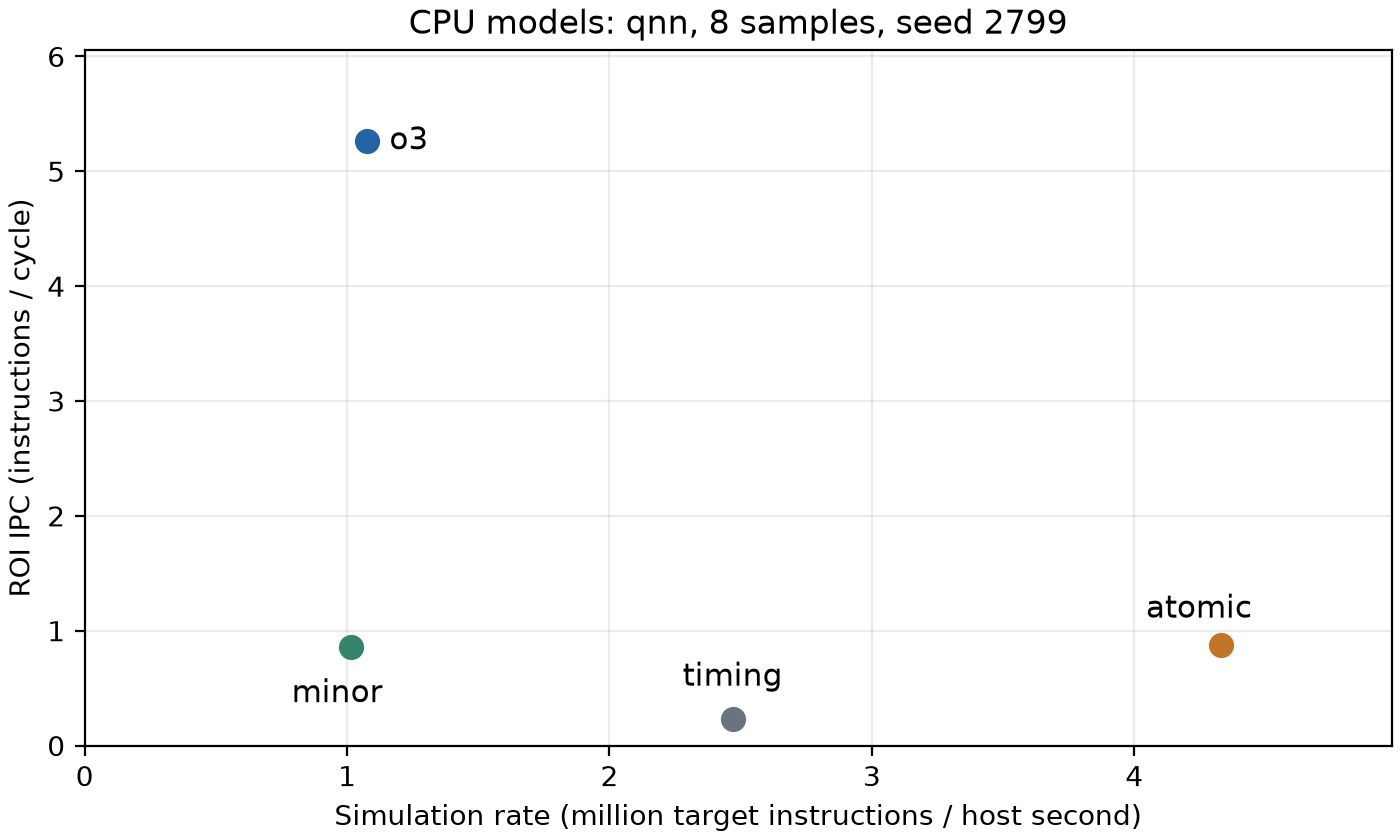
\includegraphics[width=0.90\textwidth]{task3_lab1_cpu_seed2799.png}
\caption{四模型的仿真速率与 ROI IPC，数据来自本次任务 3 CSV}\label{fig:cpu}
\end{figure}

\paragraph{Atomic 与 Minor 接近，为何不能替换？}
Atomic 的 IPC 为 0.871679，Minor 为 0.861559，数值接近的原因并不相同。Atomic 采用原子访存，本配置关闭指令与数据访问停顿模拟；Minor 具有顺序流水线及真实时序交互。两者都在此负载上得到接近 1 的平均 IPC，并不意味着对 Cache 延迟或队列资源变化会作出相同响应。任务 4 将进一步检验这种响应。

\paragraph{Timing 与 Atomic 都逐条执行，为何差很多？}
二者的 L1D 失效率均约 0.7846\%，而 Timing 的周期为 Atomic 的 3.77 倍。Timing 等待实际访存响应，命中也有非零延迟；Atomic 在当前设置下不将这些延迟计为访存停顿。

\begin{table}[H]\centering\small
\caption{任务 3：失效、合并与新 MSHR 请求}\label{tab:mshr}
\begin{tabular}{lrrrr}\toprule
模型 & L1D 失效率 & 失效次数 & 新 MSHR 数 & MSHR MPKI \\\midrule
atomic & 0.7846\% & 12\,827 & 0 & 0.000000 \\
timing & 0.7846\% & 12\,827 & 12\,827 & 2.211260 \\
minor & 0.7851\% & 12\,844 & 12\,828 & 2.211432 \\
o3 & 12.3249\% & 202\,290 & 12\,828 & 2.211432 \\
\bottomrule\end{tabular}\end{table}
表~\ref{tab:mshr} 中 O3 的 202\,290 次失效对应 12\,828 个新 MSHR，平均每个新请求对应 15.77 次失效访问，其中后续访问合并到已有请求。失效表示访问时数据尚未在 L1 中；如果同一块已有请求，则后续 load 可附加到已有 MSHR，而不再次向下一级取块。Atomic 的 MSHR 数为零源于原子访问路径。代码中的 \texttt{l1d\_mlp} 用失效次数除以新 MSHR 数，本文将它解释为合并比。

\paragraph{O3 的约六倍吞吐来自哪些机制？}
一是较宽的发射能力，本配置 O3 可每周期发射最多 8 条，Minor 的上限为 2；二是乱序调度可以绕过暂时缺少操作数的指令，提前执行独立工作；三是支持在途访存与计算重叠，既可为不同块并发请求，也可为相同块合并等待者。这些机制共同提高有效吞吐。Minor 的顺序发射和依赖约束限制了调度自由度。

\subsection{任务四：模型是否会选错 Cache}
\begin{table}[H]\centering\small
\caption{任务 4：qnn 上的 L1D 选择；节省为 $(C_{16}-C_{128})/C_{16}$}\label{tab:fid}
\begin{tabular}{lrrrl}\toprule
模型 & 16 KiB 周期 & 128 KiB 周期 & 周期节省 & 选择与参考对照 \\\midrule
timing & 23\,442\,263 & 28\,140\,926 & -20.044\% & 16 KiB（与参考相反） \\
minor & 6\,665\,404 & 6\,660\,951 & 0.067\% & 近似相同（漏判收益） \\
o3 & 1\,076\,306 & 905\,805 & 15.841\% & 128 KiB（参考） \\
\bottomrule\end{tabular}\end{table}
三种结论分别是：Timing 选择小 Cache，Minor 认为近似相同，O3 选择大 Cache。O3 的大 Cache 节省 15.84\% 周期，速度为小 Cache 的 1.188 倍；Minor 的 0.0668\% 改善低于阈值，按无差别处理。

\begin{table}[H]\centering\small
\caption{任务 4 的 Cache 行为与 IPC}\label{tab:fidmem}
\begin{tabular}{llrrr}\toprule
模型 & L1D & 失效率 & 新 MSHR 数 & IPC \\\midrule
timing & 16 KiB & 0.7851\% & 12\,834 & 0.247449 \\
timing & 128 KiB & 0.0009\% & 14 & 0.206133 \\
minor & 16 KiB & 0.7854\% & 12\,835 & 0.870280 \\
minor & 128 KiB & 0.0016\% & 14 & 0.870862 \\
o3 & 16 KiB & 12.3124\% & 12\,834 & 5.389514 \\
o3 & 128 KiB & 0.0139\% & 14 & 6.403990 \\
\bottomrule\end{tabular}\end{table}
\texttt{scaled\_latency()} 使 16 KiB 的 L1D 延迟参数为 2，128 KiB 为 5。大 Cache 提供更少失效，但付出更长命中延迟。对 Timing，可以用
\[
AMAT\approx t_{\mathrm{hit}}+m\,p_{\mathrm{extra}}
\]
理解这种权衡。它两次均执行约 163.5 万次 L1D 访问，增加的访问延迟无法像宽乱序核那样被充分隐藏，因此减少约 1.28 万个新失效请求后，总周期仍增加 20.04\%。它的结论适用于自己的阻塞式执行语义，却与本实验高性能核心的 O3 参考排序相反。

Minor 的大 Cache 同样将新请求降至 14 个，但其顺序调度、依赖与执行资源限制仍然存在，整体收益未抵过新增延迟等成本，最终只有 0.0668\% 的差别。它漏掉了 O3 上明显的大 Cache 收益。

O3 的新请求从 12\,834 降至 14，降低了反复从 L2 取权重及等待数据的成本。其 load-queue-full 事件从 188\,369 降至 17\,776，说明相关资源压力减轻。值得注意的是，平均 load-to-use 从 4.82 升到 6.50 周期，执行却更快：单次平均延迟并不决定乱序核吞吐，等待能否重叠和队列能否持续接纳工作同样重要。减少 MSHR 分配减少了数据等待及在途资源占用。

这组结果支持后续以 O3 研究 Cache、流水线及加速器的时序收益。只关心功能、校验和或指令数时，可在确认二进制和完成路径一致后使用 Atomic 提高效率。

\subsection{任务五：规模稳定性与仿真成本}
实验前预计 IPC 随样本数上升后在 8 样本附近稳定，主机成本近似为固定开销与线性样本成本之和。表~\ref{tab:scale} 使用串行实测，IPC 差值以 32 样本为参照。
\begin{table}[H]\centering\scriptsize
\caption{任务 5：ROI 计数与主机成本；时间单位为秒}\label{tab:scale}
\begin{tabular}{rrrrrrr}\toprule
样本 & 指令数 & 周期数 & IPC & ROI 主机 & 全程实际 & IPC 差值 \\\midrule
2 & 1\,450\,200 & 275\,460 & 5.264648 & 1.19 & 2.393 & -0.0862\% \\
4 & 2\,900\,385 & 550\,767 & 5.266083 & 2.36 & 3.506 & -0.0589\% \\
8 & 5\,800\,766 & 1\,101\,594 & 5.265793 & 4.64 & 5.796 & -0.0645\% \\
16 & 11\,601\,526 & 2\,202\,119 & 5.268347 & 9.18 & 10.295 & -0.0160\% \\
32 & 23\,203\,018 & 4\,403\,527 & 5.269189 & 18.55 & 19.761 & 0.0000\% \\
\bottomrule\end{tabular}\end{table}
\begin{figure}[H]\centering
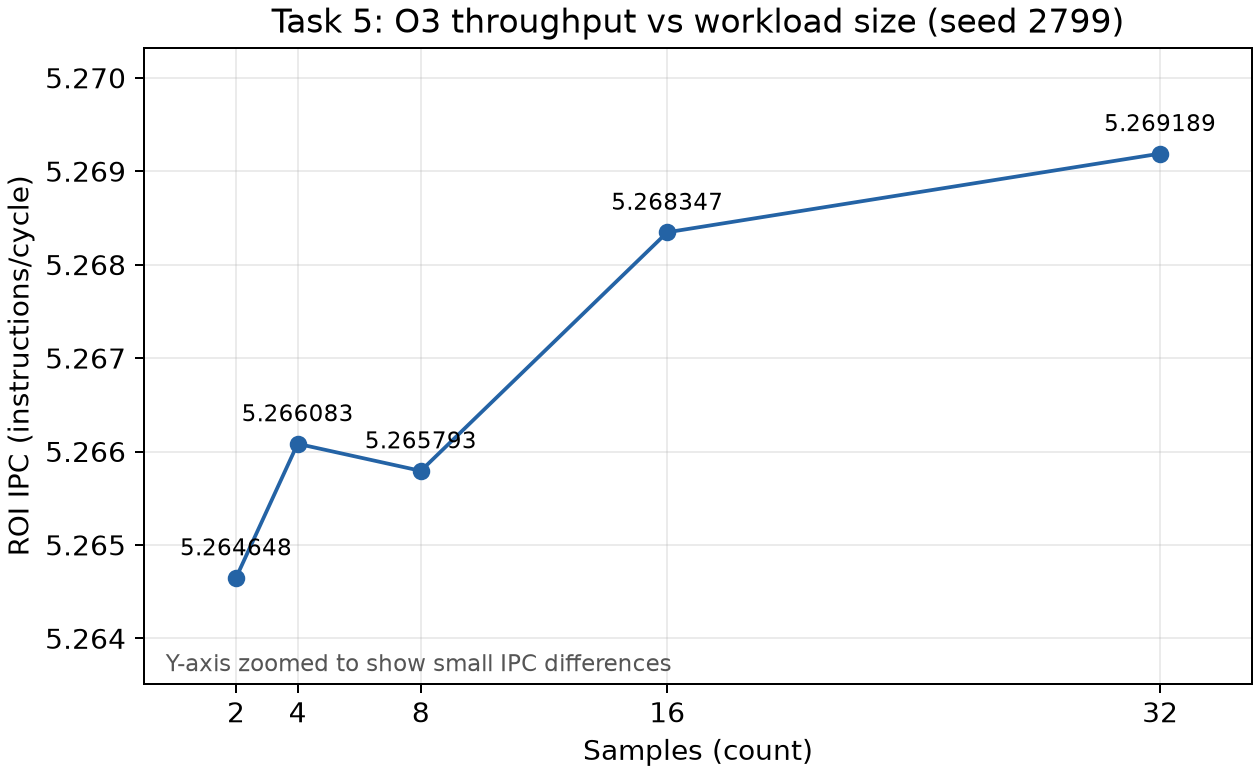
\includegraphics[width=0.87\textwidth]{task5_lab1_scale_seed2799_ipc.png}
\caption{IPC 随样本数变化；纵轴放大以呈现微小变化}\label{fig:scaleipc}
\end{figure}
图~\ref{fig:scaleipc} 不是严格单调，4 样本的 IPC 略高于 8 样本，但全体极差只有约 0.0863\%。按 0.1\% 规则，最小的 2 样本已与 32 样本近似相同，稳定出现得比预测更早。所有规模的 ROI L1I 失效均为 9 次；随着重复增加，早期固定效应的占比下降。对于低于阈值的起伏，不再逐点归因。

\begin{figure}[H]\centering
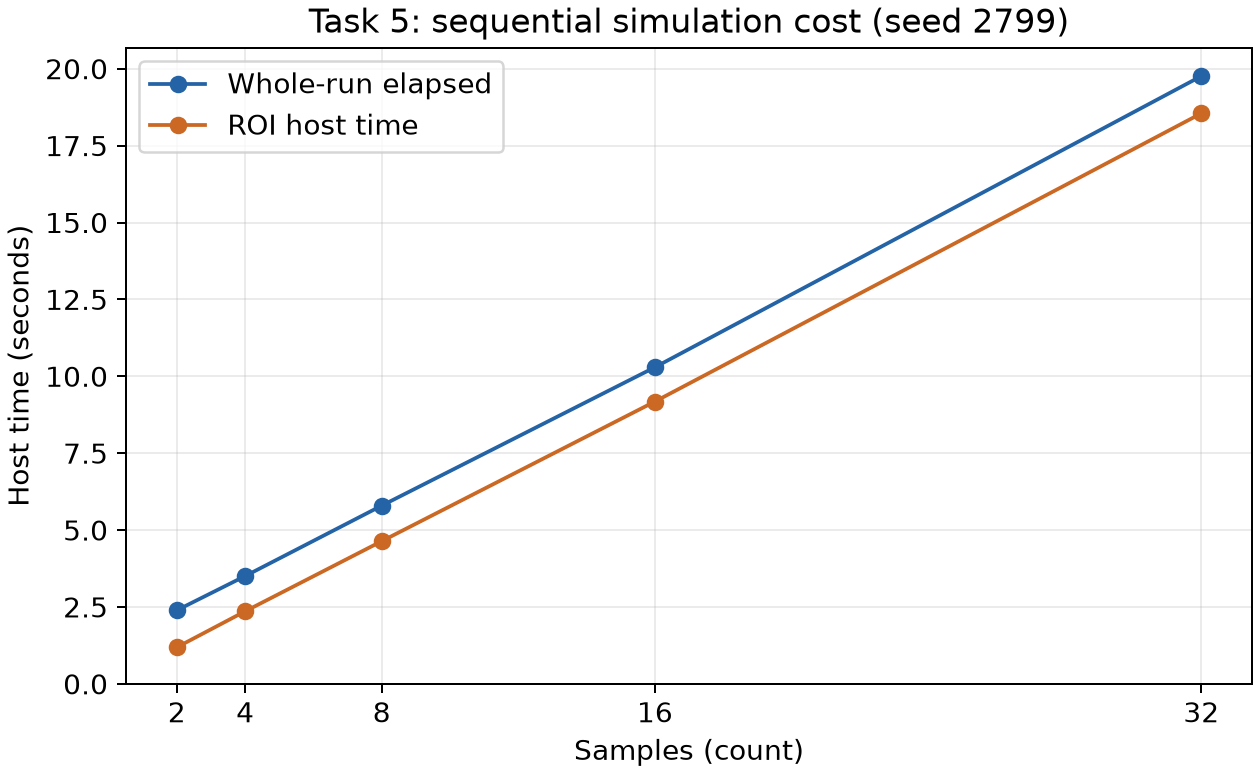
\includegraphics[width=0.87\textwidth]{task5_lab1_scale_seed2799_host_time.png}
\caption{主机耗时随样本数变化；蓝线包括模拟器进程建立及退出}\label{fig:scaletime}
\end{figure}
图~\ref{fig:scaletime} 中 ROI 主机时间近似与样本数成正比，全程时间还包含固定成本，可写为
\[
T_{\mathrm{host}}(n)\approx T_0+nT_s.
\]
8 到 32 样本的全程时间比为 $19.760948/5.795646\approx3.410$，小于 4；ROI 时间比为 $18.55/4.64\approx3.998$，接近 4，符合预测。\texttt{wall\_seconds} 是包围 gem5 子进程测得的实际等待时间；\texttt{hostSeconds} 三段相加不包括该进程运行前后的全部固定成本，因此扫描预算采用前者。

后续仍选 \textbf{8 样本}作为保守默认。它的 IPC 已稳定，成本为 4.64 s 的 ROI 主机时间、5.796 s 的全程时间；在当前配置下 2 样本更省，但新配置仍可能改变稳定所需的重复次数。更多样本提供更长观测，不等同于自动得到更真实的负载。

对于题设的 20 个配置点和 8 个可并行核心，若单点耗时相近且内存足够，需三批完成：
\[
T_{\mathrm{scan}}\approx\left\lceil\frac{20}{8}\right\rceil T_{\mathrm{run}}.
\]
8 样本约为 $3\times5.795646=17.39$ s；2 样本约 7.18 s；32 样本约 59.28 s。实际并发会共享主机资源，且不同配置耗时不同，这里仅作预算估计。

不能随意缩小会改变工作集的程序。例如将大矩阵缩成小矩阵，可能使原本超出 L1 的数据完全驻留 L1，从而消除研究所需的容量失效。qnn 减少样本数保持网络尺寸和权重数组不变，主要缩短重复次数，更容易保留单次推理的存储行为。

\subsection{任务六（选做）：依赖访存负载的对照}
\begin{lstlisting}[language=C,caption={pchase 的测量循环}]
uint32_t p = 0;
ROI_BEGIN();
for (long k = 0; k < accesses; k++)
    p = next[p];
ROI_END();
\end{lstlisting}
循环中下一次地址必须等待上次 load 的结果，因此宽发射和乱序调度无法并发执行这条依赖链。独立的循环控制仍可重叠，但不能消除链上的等待。实验前预计 O3 与 Minor 更接近，三个模型更可能同意，同时猜测增加命中延迟会使 O3 偏向 16 KiB。

\begin{table}[H]\centering\small
\caption{任务 6：pchase 的 Cache 排序}\label{tab:pchase}
\begin{tabular}{lrrrl}\toprule
模型 & 16 KiB 周期 & 128 KiB 周期 & 周期节省 & 选择 \\\midrule
timing & 7\,737\,336 & 7\,263\,838 & 6.12\% & 128 KiB \\
minor & 4\,316\,977 & 3\,767\,904 & 12.72\% & 128 KiB \\
o3 & 4\,339\,959 & 3\,865\,761 & 10.93\% & 128 KiB \\
\bottomrule\end{tabular}\end{table}
三种模型均选择 128 KiB，支持排序趋同的预测，但与“小 Cache 更好”的预测相反。O3 在两个容量下分别比 Minor 多用 0.53\% 和 2.60\% 的周期，qnn 上的约六倍优势消失；Timing 的总周期仍约为 O3 的 1.78 和 1.88 倍。

\begin{table}[H]\centering\small
\caption{任务 6 的失效与新 MSHR 请求}\label{tab:pchasemem}
\begin{tabular}{llrrr}\toprule
模型 & L1D & 失效率 & 失效次数 & 新 MSHR 数 \\\midrule
timing & 16 KiB & 94.097\% & 188\,194 & 188\,194 \\
timing & 128 KiB & 51.851\% & 103\,703 & 103\,703 \\
minor & 16 KiB & 94.097\% & 188\,193 & 188\,193 \\
minor & 128 KiB & 51.851\% & 103\,702 & 103\,702 \\
o3 & 16 KiB & 94.097\% & 188\,193 & 188\,193 \\
o3 & 128 KiB & 51.850\% & 103\,701 & 103\,701 \\
\bottomrule\end{tabular}\end{table}
O3 的每次失效均对应新 MSHR，说明同块合并没有发挥作用。原因是依赖链串行发出 load，上一块取回后才知道下一地址；随机性使步长预测困难，依赖性则直接限制同时在途的链上 load。

大 Cache 将 O3 失效率由 94.10\% 降至 51.85\%，少了约 8.45 万个低层请求。尽管 256 KiB 数组放不进 128 KiB L1D，Cache 仍能保留更多块供后续随机重用。O3 平均 load-to-use 从 18.70 降至 16.33 周期，降低的等待超过增加的 L1 命中延迟，最终节省 10.93\% 周期。

对 qnn，Timing 选小、Minor 判平、O3 选大；对 pchase，三者都选大。由此可见，模型的排序保真度取决于负载的依赖、局部性和并行性。Timing 在指针追逐上的成功不推翻采用 O3 的理由，而是说明应按工作负载及设计问题验证模型适用性。

\section{思考题}
\subsection{“误差 20\%，所以模拟器没用”是否成立？}
不能仅凭绝对误差否定模拟器。绝对保真要求数值接近真机；排序保真要求设计优劣顺序一致。任务 6 中 Timing 的绝对周期远大于 O3，却同样判断 128 KiB 更好，仍可为该问题提供方向。任务 4 中 Timing 则把 O3 上节省 15.84\% 周期的方案判成变慢 20.04\%，会导致反向选择。实验真正关心的是简化是否保留影响当前决策的机制。

\subsection{仿真真实运行一秒的程序需要多久？}
按题设 2 GHz、IPC 为 1，目标一秒约执行 $2\times10^9$ 条指令。若速率为 $3\times10^5$ 条/主机秒，则
\[
T_{\mathrm{sim}}=\frac{2\times10^9}{3\times10^5}
\approx6666.7\ \mathrm{s}=111.1\ \mathrm{min}\approx1.85\ \mathrm{h}.
\]
本次任务 3 的 O3 速率为 1\,076\,973 条/秒，按该测量速率机械外推约需 1\,857 s，即 31.0 min。对数十个设计点，长程序逐指令详细仿真成本很高。可采用 SimPoint 选择代表性阶段并按权重汇总，用 checkpoint 保存状态后从目标阶段恢复，先用快速模型快进再切换详细模型，或用 FPGA 原型加速执行。

\subsection{限制样本数与 \texttt{--maxinsts} 的差异}
限制样本数按算法语义结束，保留完整的输入生成、推理及结果更新；工作量减少的含义明确。\texttt{--maxinsts N} 则从执行起点累计到指令上限即停，可能截在初始化内部、某层推理中间或一次输出之前。以本实验为例，初始化已超过 112 万条指令，若直接设置 100 万条，甚至还没有进入 ROI。算法或 ISA 优化改变指令数后，相同上限还会对应不同的有效工作量。随意截断更容易比较不同阶段从而出错。

\subsection{ROI 排除权重初始化是否影响预热公平性？}
ROI 重置统计但保留缓存状态，初始化写过权重会影响推理开始时的驻留状态。对于反复使用已初始化权重的部署，这是有意义的运行场景；对于只做一次推理的端到端延迟，初始化和装载本身也属于成本。不同容量在相同初始化流程后形成不同驻留状态，是程序与存储层次交互的结果。

\section{总结}
实验完整建立了从二进制、配置、ROI、统计块到结果 CSV 的测量流程。三段统计揭示初始化对整体 IPC 的显著影响；布局实验说明微小代码位置变化可以带来约三倍的周期差异；模型实验表明绝对 IPC 接近不足以保证设计排序一致；规模实验给出了稳定性和成本之间的具体取舍；指针追逐则说明同一模型的排序保真度会随负载改变。

\subsection*{模型选择声明（不超过 300 字）}
后续实验默认采用 O3、qnn 8 样本和种子 2799，以 ROI 周期比较方案。O3 能反映宽发射、乱序调度与访存重叠；在本次 Cache 比较中，Timing 给出反向结论，Minor 漏判明显收益。8 样本 IPC 已稳定，全程约 5.80 秒，20 点、8 核预算约 17.39 秒。只检验功能或指令数时可改用 Atomic。O3 仍依赖参数、ROI 和负载代表性。

\appendix
\clearpage
\section{实验自动化源代码}
下面直接嵌入用于复现实验和生成图表的自动化代码。共享的基准程序和 gem5 框架沿用项目实现。
\subsection{主运行脚本 run.sh}
脚本负责参数解析、构建、单点与扫描任务调度。
\begin{lstlisting}[language=bash]
#!/usr/bin/env bash
set -euo pipefail

# Keep paths (including the simulated argv) consistent from any working directory.
LAB_DIR="$(cd -- "$(dirname -- "${BASH_SOURCE[0]}")" && pwd -P)"
RESULT_DIR="$LAB_DIR/results"

usage() {
  cat<<'EOF'
Usage:
  ./run.sh TASK [--seed NUMBER]

Tasks:
  task1     Run qnn with 8 samples
  task2b    Run qnn with 64 samples
  task2c    Compare 4 binaries with 8 samples
  task3     Sweep four CPU models; save ROI metrics and scatter plot
  task3plot Plot the existing Task 3 CSV without rerunning simulations
  task4     Compare 16kB and 128kB L1D on timing, minor, and o3
  task5     Run 2, 4, 8, 16, 32 samples sequentially; save CSV and plots
  task6     Compare 16kB and 128kB L1D using dependent pointer chasing
  symbols   Inspect dot_i8 in the existing binaries; no simulation
  icache    Export I-Cache counters from existing runs for this seed
  all       Run task1, task2b, task2c, task3, task4, task5, and task6

Options:
  --seed NUMBER     Random seed; default: 2799
  -h, --help        Show this help

Results:
  out/      Raw simulator outputs and logs
  results/   Readable statistics summaries

Rerunning the same task and seed replaces its previous output.
EOF
}

TASK=""
SEED=2799

while (( $# > 0 )); do
  case "$1" in
    task1|task2b|task2c|task3|task3plot|task4|task5|task6|symbols|icache|all)
      if [[ -n "$TASK" ]]; then
        printf 'ERROR: Choose only one task.\n' >&2
        exit 2
      fi
      TASK="$1"
      shift
      ;;

    --seed)
      if (( $# < 2 )); then
        printf 'ERROR: --seed requires a number.\n' >&2
        exit 2
      fi
      SEED="$2"
      shift 2
      ;;

    -h|--help)
      usage
      exit 0
      ;;

    *)
      printf 'ERROR: Unknown argument: %s\n' "$1" >&2
      usage >&2
      exit 2
      ;;
  esac
done

if [[ -z "$TASK" ]]; then
  usage >&2
  exit 2
fi

if [[ ! "$SEED" =~ ^[0-9]{4}$ ]]; then
  printf 'ERROR: seed must be an 4 digits integer number.\n' >&2
  exit 2
fi

SEED_DECIMAL=$((10#$SEED))

cd "$LAB_DIR"
source ../setup.sh

run_case() {
  mkdir -p "$RESULT_DIR"
  local label="$1"
  local binary="$2"
  local samples="$3"
  local blocks="$4"

  local block
  local name="$label"
  if [[ "$label" == task2c ]]; then
    name="${label}_${binary}"
  fi

  local out_dir="out/${name}_o3_n${samples}_seed${SEED}"
  local summary="results/${name}_o3_n${samples}_seed${SEED}.txt"

  mkdir -p "$out_dir"
  "$GEM5_BIN" \
    --outdir="$out_dir" \
    framework/cssys_se.py \
    --cmd "bench/bin/riscv/$binary" \
    --options "$samples $SEED_DECIMAL" \
    --cpu o3 \
    2>&1 | tee "$out_dir/run.log"

  {
    for (( block=0; block<blocks; block++ )); do
      if (( block > 0 )); then
        printf '\n'
      fi
      printf 'Statistics block %s:\n' "$block"
      python framework/stats.py "${out_dir}/stats.txt" "$block"
    done
  } > "$summary"

  printf 'Saved summary: %s\n' "$summary"
}

export_icache() {
  local -a stats_files=()
  local path
  for path in out/*_seed"$SEED"/stats.txt; do
    [[ -f "$path" ]] && stats_files+=("$path")
  done
  if (( ${#stats_files[@]} == 0 )); then
    printf 'ERROR: no statistics found for seed %s.\n' "$SEED" >&2
    return 1
  fi
  python "$LAB_DIR/icache_report.py" \
    --output "$RESULT_DIR/task2c_icache_seed${SEED}.csv" "${stats_files[@]}"
}

task1() {
  run_case task1 qnn 8 3
}

task2b() {
  run_case task2b qnn 64 3
}

task2c() {
  local binary
  local blocks

  for binary in qnn qnn_noroi qnn_noalign qnn_noalign_noroi; do
    case "$binary" in
      *_noroi)    blocks=1 ;;
      *)          blocks=3 ;;
    esac
    run_case task2c "$binary" 8 "$blocks"
  done

  inspect_dot_i8
}

task3() {
  local name="task3_lab1_cpu_seed${SEED}"
  python framework/sweep.py \
    --name "$name" \
    --bench qnn --bench-args "8 $SEED_DECIMAL" \
    --vary cpu=atomic,timing,minor,o3 --jobs 4

  python framework/report.py "$RESULT_DIR/${name}.csv" \
    insts cycles ipc host_seconds host_inst_rate \
    l1d_miss_rate l1d_mshr_mpki \
    | tee "$RESULT_DIR/${name}.txt"

  plot_task3
}

plot_task3() {
  local name="task3_lab1_cpu_seed${SEED}"
  uv run --no-project --with matplotlib python "$LAB_DIR/task3_plot.py" \
    --input "$RESULT_DIR/${name}.csv" \
    --output "$RESULT_DIR/${name}.png" \
    --report-output "$LAB_DIR/lab-report/images/${name}.png"
}

task4() {
  local name="task4_lab1_fid_seed${SEED}"
  python framework/sweep.py \
    --name "$name" \
    --bench qnn --bench-args "8 $SEED_DECIMAL" \
    --vary cpu=timing,minor,o3 --vary l1d-size=16kB,128kB --jobs 6

  python framework/report.py "$RESULT_DIR/${name}.csv" \
    cycles ipc l1d_miss_rate l1d_mshr_mpki \
    | tee "$RESULT_DIR/${name}.txt"
}

task5() {
  local table="$RESULT_DIR/task5_lab1_scale_seed${SEED}.csv"
  python "$LAB_DIR/task5_scale.py" run \
    --seed "$SEED" --gem5 "$GEM5_BIN" --output "$table"
  # uv keeps the plotting dependency separate from the gem5 build environment.
  uv run --no-project --with matplotlib python "$LAB_DIR/task5_scale.py" plot \
    --input "$table"
}

task6() {
  local name="task6_lab1_fid_pchase_seed${SEED}"
  python framework/sweep.py \
    --name "$name" \
    --bench pchase --bench-args "256 200000 $SEED_DECIMAL" \
    --vary cpu=timing,minor,o3 --vary l1d-size=16kB,128kB --jobs 6

  python framework/report.py "$RESULT_DIR/${name}.csv" \
    insts cycles ipc l1d_miss_rate l1d_mshr_mpki \
    | tee "$RESULT_DIR/${name}.txt"
}

# Run a matching RISC-V utility locally, or use the benchmark Docker image.
riscv_tool() {
  local utility="$1"
  shift
  local prefix
  local -a docker_cmd=(docker)

  if [[ -n "${CROSS:-}" ]]; then
    "${CROSS}${utility}" "$@"
    return
  fi

  for prefix in riscv64-linux-gnu- riscv64-unknown-linux-gnu-; do
    if command -v "${prefix}${utility}" >/dev/null 2>&1; then
      "${prefix}${utility}" "$@"
      return
    fi
  done

  if [[ "$(uname -s)" == Darwin ]] && command -v colima >/dev/null 2>&1; then
    docker_cmd+=(--context colima-cssys)
  fi

  "${docker_cmd[@]}" run --rm \
    --mount "type=bind,source=$LAB_DIR/../bench,target=/bench,readonly" \
    --workdir /bench \
    cssys-riscv-toolchain:bookworm \
    "riscv64-linux-gnu-${utility}" "$@"
}

inspect_dot_i8() {
  local binary symbols address
  local table="$RESULT_DIR/task2c_dot_i8-addresses.csv"
  local disassembly="$RESULT_DIR/task2c_dot_i8-disassembly.txt"

  mkdir -p "$RESULT_DIR"
  # Check all inputs before replacing the previous inspection results.
  for binary in qnn qnn_noroi qnn_noalign qnn_noalign_noroi; do
    if [[ ! -f "bench/bin/riscv/$binary" ]]; then
      printf 'ERROR: missing %s; run task2c to build the binaries.\n' "$binary" >&2
      return 1
    fi
  done

  printf 'binary,function_address_hex,function_address_mod64\n' > "$table"
  : > "$disassembly"
  for binary in qnn qnn_noroi qnn_noalign qnn_noalign_noroi; do
    # Utilities use paths relative to bench, both locally and in Docker.
    symbols=$(cd bench && riscv_tool nm "bin/riscv/$binary")
    address=$(awk '$3 == "dot_i8" { print $1 }' <<< "$symbols")
    if [[ ! "$address" =~ ^[0-9a-fA-F]+$ ]]; then
      printf 'ERROR: could not find one dot_i8 symbol in %s.\n' "$binary" >&2
      return 1
    fi
    printf '%s,0x%s,%d\n' "$binary" "$address" "$((16#$address % 64))" >> "$table"
    printf '\n=== %s ===\n' "$binary" >> "$disassembly"
    (cd bench && riscv_tool objdump -d --disassemble=dot_i8 "bin/riscv/$binary") \
      >> "$disassembly"
  done
  cat "$table"
  printf 'Saved disassembly: %s\n' "$disassembly"
}

# Build the binaries needed by the selected task.
case "$TASK" in
  task1|task2b|task3|task4|task5)
    ../bench/build.sh bin/riscv/qnn
    ;;
  task2c)
    ../bench/build.sh bin/riscv/qnn bin/riscv/qnn_noroi noalign
    ;;
  task6)
    ../bench/build.sh bin/riscv/pchase
    ;;
  all)
    ../bench/build.sh bin/riscv/qnn bin/riscv/qnn_noroi noalign bin/riscv/pchase
    ;;
esac

# Execute the selected task.
case "$TASK" in
  task1)  task1 ;;
  task2b) task2b ;;
  task2c) task2c ;;
  task3) task3 ;;
  task3plot) plot_task3 ;;
  task4) task4 ;;
  task5) task5 ;;
  task6) task6 ;;
  symbols) inspect_dot_i8 ;;
  icache) export_icache ;;
  all)
    task1
    task2b
    task2c
    task3
    task4
    task5
    task6
    ;;
esac

case "$TASK" in
  task1|task2b|task2c|all) export_icache ;;
esac

rm -rf m5out
\end{lstlisting}

\subsection{任务三散点图 task3\_plot.py}
运行器在任务 3 扫描后自动调用该绘图脚本，也可使用 \texttt{task3plot} 只读取已有 CSV。横轴是每主机秒模拟的目标指令数（以百万为单位），纵轴是 ROI IPC，四个点直接标注模型名。
\begin{lstlisting}[language=Python]
"""Plot Task 3 CPU throughput against host simulation rate from its CSV."""

import argparse
import csv
from pathlib import Path
import shutil

import matplotlib
matplotlib.use("Agg")
import matplotlib.pyplot as plt


def main():
    parser = argparse.ArgumentParser(description=__doc__)
    parser.add_argument("--input", type=Path, required=True)
    parser.add_argument("--output", type=Path, required=True)
    parser.add_argument("--report-output", type=Path, required=True)
    args = parser.parse_args()
    with args.input.open(newline="", encoding="utf-8") as stream:
        rows = list(csv.DictReader(stream))
    models = ("atomic", "timing", "minor", "o3")
    if len(rows) != 4 or {row["cpu"] for row in rows} != set(models):
        raise ValueError("Expected exactly one CSV row for each of the four CPU models")
    points = {}
    for row in rows:
        if row.get("error"):
            raise ValueError(f"Simulation failed for {row['cpu']}: {row['error']}")
        rate, ipc = float(row["host_inst_rate"]), float(row["ipc"])
        if rate <= 0 or ipc <= 0:
            raise ValueError(f"Expected positive rate and IPC for {row['cpu']}")
        points[row["cpu"]] = (rate / 1e6, ipc)

    colors = {"atomic": "#c27528", "timing": "#6b7280",
              "minor": "#33846a", "o3": "#2463a5"}
    offsets = {"atomic": (-8, 10), "timing": (0, 12),
               "minor": (-5, -20), "o3": (15, -3)}
    fig, ax = plt.subplots(figsize=(7, 4.2), layout="constrained")
    for model in models:
        x, y = points[model]
        ax.scatter(x, y, s=65, color=colors[model], zorder=3)
        ax.annotate(model, (x, y), xytext=offsets[model],
                    textcoords="offset points", ha="center", fontsize=11)
    ax.set(
        xlabel="Simulation rate (million target instructions / host second)",
        ylabel="ROI IPC (instructions / cycle)",
        title=f"CPU models: qnn, 8 samples, seed {args.input.stem.rsplit('_seed', 1)[-1]}",
        xlim=(0, max(x for x, _ in points.values()) * 1.15),
        ylim=(0, max(y for _, y in points.values()) * 1.15),
    )
    ax.grid(alpha=0.25)
    args.output.parent.mkdir(parents=True, exist_ok=True)
    fig.savefig(args.output, dpi=200)
    plt.close(fig)
    args.report_output.parent.mkdir(parents=True, exist_ok=True)
    if args.output.resolve() != args.report_output.resolve():
        shutil.copy2(args.output, args.report_output)
    print(f"Saved scatter plot: {args.output}")
    print(f"Report image: {args.report_output}")


if __name__ == "__main__":
    main()
\end{lstlisting}

\subsection{规模扫描与绘图 task5\_scale.py}
该脚本在每种规模运行完整 gem5 子进程，读取三个统计块，将 ROI 计数、分段主机时间以及包围子进程的实际耗时分别保存。
\begin{lstlisting}[language=Python]
"""Run the workload-size experiment, or plot its saved measurements."""

import argparse
import csv
from pathlib import Path
import subprocess
import sys
import time

LAB_DIR = Path(__file__).resolve().parent
sys.path.insert(0, str(LAB_DIR.parent / "framework"))
from stats import parse_blocks, summarize


def run(args):
    rows = []
    for samples in (2, 4, 8, 16, 32):
        name = f"task5_o3_n{samples}_seed{args.seed}"
        out_dir = Path("out") / name
        (LAB_DIR / out_dir).mkdir(parents=True, exist_ok=True)
        command = [
            args.gem5, f"--outdir={out_dir}", "framework/cssys_se.py",
            "--cmd", "bench/bin/riscv/qnn", "--options",
            f"{samples} {int(args.seed, 10)}", "--cpu", "o3",
        ]
        print(f"Running {samples} samples (sequential)...", flush=True)
        started = time.perf_counter()
        with (LAB_DIR / out_dir / "run.log").open("w") as log:
            subprocess.run(command, cwd=LAB_DIR, stdout=log,
                           stderr=subprocess.STDOUT, check=True)
        wall_seconds = time.perf_counter() - started
        stats_path = LAB_DIR / out_dir / "stats.txt"
        blocks = parse_blocks(stats_path)
        if len(blocks) != 3:
            raise ValueError(f"{stats_path}: expected three statistics blocks")
        startup, roi, shutdown = [summarize(block) for block in blocks]
        rows.append({
            "samples": samples,
            "seed": args.seed,
            "insts": int(roi["insts"]),
            "cycles": int(roi["cycles"]),
            "ipc": roi["ipc"],
            "cycles_per_sample": roi["cycles"] / samples,
            "roi_host_seconds": roi["host_seconds"],
            "startup_host_seconds": startup["host_seconds"],
            "shutdown_host_seconds": shutdown["host_seconds"],
            "total_host_seconds": sum(block["host_seconds"] for block in
                                      (startup, roi, shutdown)),
            "wall_seconds": round(wall_seconds, 6),
            "l1i_misses": int(roi["l1i_misses"]),
            "bp_mpki": roi["bp_mpki"],
            "l1d_mshr_mpki": roi["l1d_mshr_mpki"],
            "stats_path": str(stats_path),
        })
        print(f"  IPC={roi['ipc']:.6f}; whole-run elapsed={wall_seconds:.3f}s",
              flush=True)
    # A partial/failed sweep must not replace a previous complete CSV.
    args.output.parent.mkdir(parents=True, exist_ok=True)
    with args.output.open("w", newline="", encoding="utf-8") as stream:
        writer = csv.DictWriter(stream, fieldnames=list(rows[0]))
        writer.writeheader()
        writer.writerows(rows)
    print(f"Saved measurements: {args.output}")
    print("samples       IPC     ROI host (s)    whole-run elapsed (s)")
    for row in rows:
        print(f"{row['samples']:7d} {row['ipc']:9.6f} "
              f"{row['roi_host_seconds']:16.3f} {row['wall_seconds']:24.3f}")


def plot(args):
    import matplotlib
    matplotlib.use("Agg")
    import matplotlib.pyplot as plt

    with args.input.open(newline="", encoding="utf-8") as stream:
        rows = list(csv.DictReader(stream))
    samples = [int(row["samples"]) for row in rows]
    seed = rows[0]["seed"]
    plt.rcParams.update({"font.size": 11})

    fig, ax = plt.subplots(figsize=(7, 4.3), layout="constrained")
    ipc = [float(row["ipc"]) for row in rows]
    ax.plot(samples, ipc, "o-", color="#2463a5")
    ax.set(xlabel="Samples (count)", ylabel="ROI IPC (instructions/cycle)",
           title=f"Task 5: O3 throughput vs workload size (seed {seed})",
           xticks=samples)
    ax.ticklabel_format(axis="y", style="plain", useOffset=False)
    ax.grid(alpha=0.25)
    for x, y in zip(samples, ipc):
        ax.annotate(f"{y:.6f}", (x, y), xytext=(0, 9),
                    textcoords="offset points", ha="center", fontsize=9)
    ax.margins(x=0.1, y=0.25)
    ax.text(0.02, 0.02, "Y-axis zoomed to show small IPC differences",
            transform=ax.transAxes, fontsize=9, color="#555555")
    path = args.input.with_name(args.input.stem + "_ipc.png")
    fig.savefig(path, dpi=180)
    plt.close(fig)
    print(f"Saved plot: {path}")

    fig, ax = plt.subplots(figsize=(7, 4.3), layout="constrained")
    for key, label, color in (
        ("wall_seconds", "Whole-run elapsed", "#2463a5"),
        ("roi_host_seconds", "ROI host time", "#ca6824"),
    ):
        ax.plot(samples, [float(row[key]) for row in rows], "o-",
                label=label, color=color)
    ax.set(xlabel="Samples (count)", ylabel="Host time (seconds)",
           title=f"Task 5: sequential simulation cost (seed {seed})",
           xticks=samples, ylim=(0, None))
    ax.grid(alpha=0.25)
    ax.legend()
    path = args.input.with_name(args.input.stem + "_host_time.png")
    fig.savefig(path, dpi=180)
    plt.close(fig)
    print(f"Saved plot: {path}")


def main():
    parser = argparse.ArgumentParser(description=__doc__)
    commands = parser.add_subparsers(dest="command", required=True)
    runner = commands.add_parser("run")
    runner.add_argument("--seed", required=True)
    runner.add_argument("--gem5", required=True)
    runner.add_argument("--output", type=Path, required=True)
    runner.set_defaults(action=run)
    plotter = commands.add_parser("plot")
    plotter.add_argument("--input", type=Path, required=True)
    plotter.set_defaults(action=plot)
    args = parser.parse_args()
    args.action(args)


if __name__ == "__main__":
    main()
\end{lstlisting}

\subsection{取指统计导出 icache\_report.py}
该脚本读取每个统计块，并为三段布局另加全程序汇总。
\begin{lstlisting}[language=Python]
"""Export per-region and whole-program instruction-fetch counters from gem5."""

import argparse
import csv
from pathlib import Path
import sys

sys.path.insert(0, str(Path(__file__).resolve().parent.parent / "framework"))
from stats import parse_blocks


COUNTERS = {
    "instructions": "simInsts",
    "cycles": "system.cpu.numCycles",
    "fetch_block_requests": "system.cpu.fetch.cacheLines",
    "icache_accesses": "system.cpu.icache.overallAccesses::total",
    "icache_misses": "system.cpu.icache.overallMisses::total",
    "icache_stall_cycles": "system.cpu.fetchStats0.icacheStallCycles",
}


def rows_for(path):
    blocks = parse_blocks(path)
    if len(blocks) not in (1, 3):
        raise ValueError(f"{path}: expected 1 or 3 statistics blocks, got {len(blocks)}")
    totals = dict.fromkeys(COUNTERS, 0)
    regions = ["whole_program"] if len(blocks) == 1 else ["startup", "roi", "shutdown"]
    for index, (block, region) in enumerate(zip(blocks, regions)):
        # Missing counters are errors, rather than misleading zero measurements.
        values = {column: int(block[key]) for column, key in COUNTERS.items()}
        for column, value in values.items():
            totals[column] += value
        yield make_row(path, region, index, values)
    if len(blocks) == 3:
        yield make_row(path, "whole_program", "all", totals)


def make_row(path, region, block, values):
    cycles = values["cycles"]
    accesses = values["icache_accesses"]
    return {
        "run": path.parent.name,
        "region": region,
        "block": block,
        **values,
        "icache_stall_percent": round(100 * values["icache_stall_cycles"] / cycles, 6) if cycles else "",
        "icache_miss_percent": round(100 * values["icache_misses"] / accesses, 6) if accesses else "",
        "stats_path": str(path.resolve()),
    }


def main():
    parser = argparse.ArgumentParser(description=__doc__)
    parser.add_argument("--output", type=Path, required=True)
    parser.add_argument("stats", type=Path, nargs="+")
    args = parser.parse_args()
    # Parse every input before replacing an existing report.
    rows = [row for path in args.stats for row in rows_for(path)]
    args.output.parent.mkdir(parents=True, exist_ok=True)
    with args.output.open("w", newline="", encoding="utf-8") as stream:
        writer = csv.DictWriter(stream, fieldnames=list(rows[0]))
        writer.writeheader()
        writer.writerows(rows)
    print(f"Saved I-Cache report: {args.output} ({len(rows)} rows)")


if __name__ == "__main__":
    main()
\end{lstlisting}

\section{运行命令与提交内容}
从本实验目录执行以下命令。运行输出直接嵌入各结果表。
\begin{lstlisting}[language=bash]
./run.sh --help
./run.sh all --seed 2799
# Individual experiments:
./run.sh task1
./run.sh task2b
./run.sh task2c
./run.sh task3
./run.sh task4
./run.sh task5
./run.sh task6
# Re-extract existing data without simulation:
./run.sh symbols
./run.sh icache
./run.sh task3plot
\end{lstlisting}
单独的任务命令适合检查与重跑某个实验；本报告使用最后一次 \texttt{all} 的结果以保持时间测量批次一致。
\end{document}
